\chapter[Capítulo 2. Marco Teórico y Fundamentos]{Estado del Arte y Marco Teórico}

El presente capítulo se centra en el  marco teórico y los fundamentos de  monitoreo vehicular denominado diagnosis vehicular. En ese contexto, se exponen las principales características de los sistemas de diagnosis vehicular como las tecnologías utilizadas para su desarrollo. Finaliza el capítulo con las conclusiones más relevantes del mismo.


\section{Generación de Diagnosis a Bordo}

\subsection{Primera Generación de Diagnosis a Bordo (OBD-I)}

Para notificar a los conductores del estado del vehículo y minimizar la contaminación atmosférica producida por el parque automovilístico, en 1987 se incluyó la primera generación de diagnosis a bordo en las nuevas producciones de vehículos vendidos, esto ocurrió en California (USA). Los vehículos tenían incorporados equipos electrónicos que ofrecían respuestas a demandas realizadas por las organizaciones americanas EPA (Environmental Protection Agency) y SAE (Society Automobile Engineering). 
Más tarde se definieron los requisitos de la primera generación de diagnosis a bordo (OBD-I), el cual ofrecía:

\begin{itemize}
\item Incorporar indicadores luminosos para informar de algún tipo de fallos al conductor.
\item Poner a disposición de los talleres de reparación un manual de códigos de fallos, para interpretar los errores leídos desde la memoria de los equipos electrónicos.
\item Incorporar a los equipos electrónicos una memoria para almacenar fallos del vehículo. 
\item Monitorizar la emisión de gases de escape y relacionar dicha emisión con los fallos de los componentes eléctricos que controlan el funcionamiento del motor.
\end{itemize}

La primera generación de OBDs fue concebida para notificar sobre el fallo de mecanismos del vehículo que contribuían a las emisiones de gases contaminantes para el medio ambiente. En este grupo de sistemas se incluían:

\begin{itemize}
\item Todos los sensores importantes del motor: temperatura de refrigeración del motor, temperatura interna del motor, posición de la mariposa, etc.
\item Sistema de medida de nivel de combustible.
\item Sistema de recirculación de los gases de escape.
\end{itemize}

La incorporación de la tecnología electrónica en el sector del automóvil permitió afrontar la necesidad de reducir la contaminación producida por los vehículos a motor, informar al conductor del estado de los mismos y reducir los tiempos para detectar fallos.

\subsection {Segunda Generación de Diagnosis a Bordo (OBD-II)}
La segunda generación de diagnosis a bordo surge de la necesidad de mejorar las prestaciones del OBD-I:

\begin {itemize}
\item Mejorar el diagnostico de los datos que ofrece el sensor de oxigeno.
\item Detección del fallo del motor.
\item Detección de oxigeno no quemado en la explosión dentro del motor lo cual permitió mejorar la eficiencia de los mismos.
\item Incorporación de equipos de diagnosis (Scantools). Al detectar fallos ocurridos en los sistemas a bordo del vehículo se genera un código para representar dicho fallo. Dicho código se memoriza en una zona de históricos en el vehículo para ser monitoreado, utilizando Scantools off-line. 
\end{itemize}

A partir de 1996 se impone de forma masiva la implementación de los OBD-II. Los vehículos de turismo y de mercancías ligeros se vieron obligados a incorporar las nuevas funcionalidades. Una particularidad de los OBD-II, es el requisito de que todos los sistemas y componentes relacionados con el sistema de expulsión de gases deben ser monitorizados para detectar cualquier mal funcionamiento que pudiera dar lugar a un incremento significativo en la emisión de gases nocivos. 
OBD-II advierte al conductor mediante  el uso de “displays”, el funcionamiento anómalo de alguno de los componentes del vehículo y proporciona los códigos significativos del tipo de fallo y de los componentes defectuosos. Los datos proporcionados por OBD-II permiten determinar con precisión el componente específico que se ha estropeado, ahorrando tiempo y costo de reparación. 
En OBD-II la luz de chequeo o displays eran presentadas de tres formas:
\begin{itemize}
\item Destellos Ocasionales: se produce un parpadeo de forma ocasional cuando el defecto de funcionamiento es momentáneo, en cambio, si el defecto es más grave el parpadeo es continuo.
\item Destellos constantes: indica que existe un problema que puede ocasionar un daño grave al motor si es que no se repara a tiempo. 
\item Indicación de fallo grave: se activa cuando se presentan problemas muy graves, y permanece activo mientras el vehículo esté funcionando.
\end{itemize}

En todos los casos de diagnosis, la información que almacena la computadora central sobre los fallos ocurridos en el automóvil, se obtiene utilizando equipos de hardware concretos y un software apropiado conocido como “Scantools”, utilizando conectores y protocolos estandarizados.
Dicha información consta de unos códigos también estandarizados, donde cada uno de ellos está asociado a la ubicación física donde se localiza e identifica el fallo.
Europa estandarizó un sistema similar a OBD-I y OBD-II conocido como EOBD-I (European On Board Diagnostics, por sus siglas en inglés). Dicho estándar se empezó a aplicar a partir del 2001, y a partir de esa fecha todos los automóviles fabricados en Europa incorporan un sistema de diagnosis a bordo para monitorizar las emisiones de gases del motor.

\subsection {Tercera Generación de Diagnosis de a Bordo (OBD-III)}


EL objetivo principal de OBD-III es el de minimizar la demora entre la detección de un fallo o funcionamiento defectuoso y la reparación del vehículo. La nueva versión deberá ser capaz de recibir la información proporcionada por OBD-II, interpretarla, enviar conclusiones a los conductores y talleres de reparación con las claves de los fallos detectados, y al mismo tiempo crear  un histórico en un centro de datos, para ser utilizados en diagnosis y diseños futuros.


En la  \textbf{Figura \ref{DenB}} se expone el concepto de OBD-III. Los fallos del vehículo son enviados  a un centro de atención al cliente que analiza los datos recibidos. El centro de atención al cliente notifica al cliente las acciones a tomar para eliminar el fallo. El centro de atención al cliente envía al taller la información necesaria para la reparación  y las pruebas posteriores una vez subsanada la avería. También existe una conexión con la central de datos donde se almacena todas las averías del vehículo de manera a obtener un historial de fallos.
OBD-III es la capacidad de comunicación del vehículo con el mundo exterior. En este sentido se están proponiendo y utilizando diferentes alternativas tecnológicas que permitan leer datos almacenados por OBD-II y enviarlos a Centros de Atención al Cliente, Centro de Datos, Servicios Móviles de Mantenimiento, etc.

\begin{figure}[H]
	\centering
		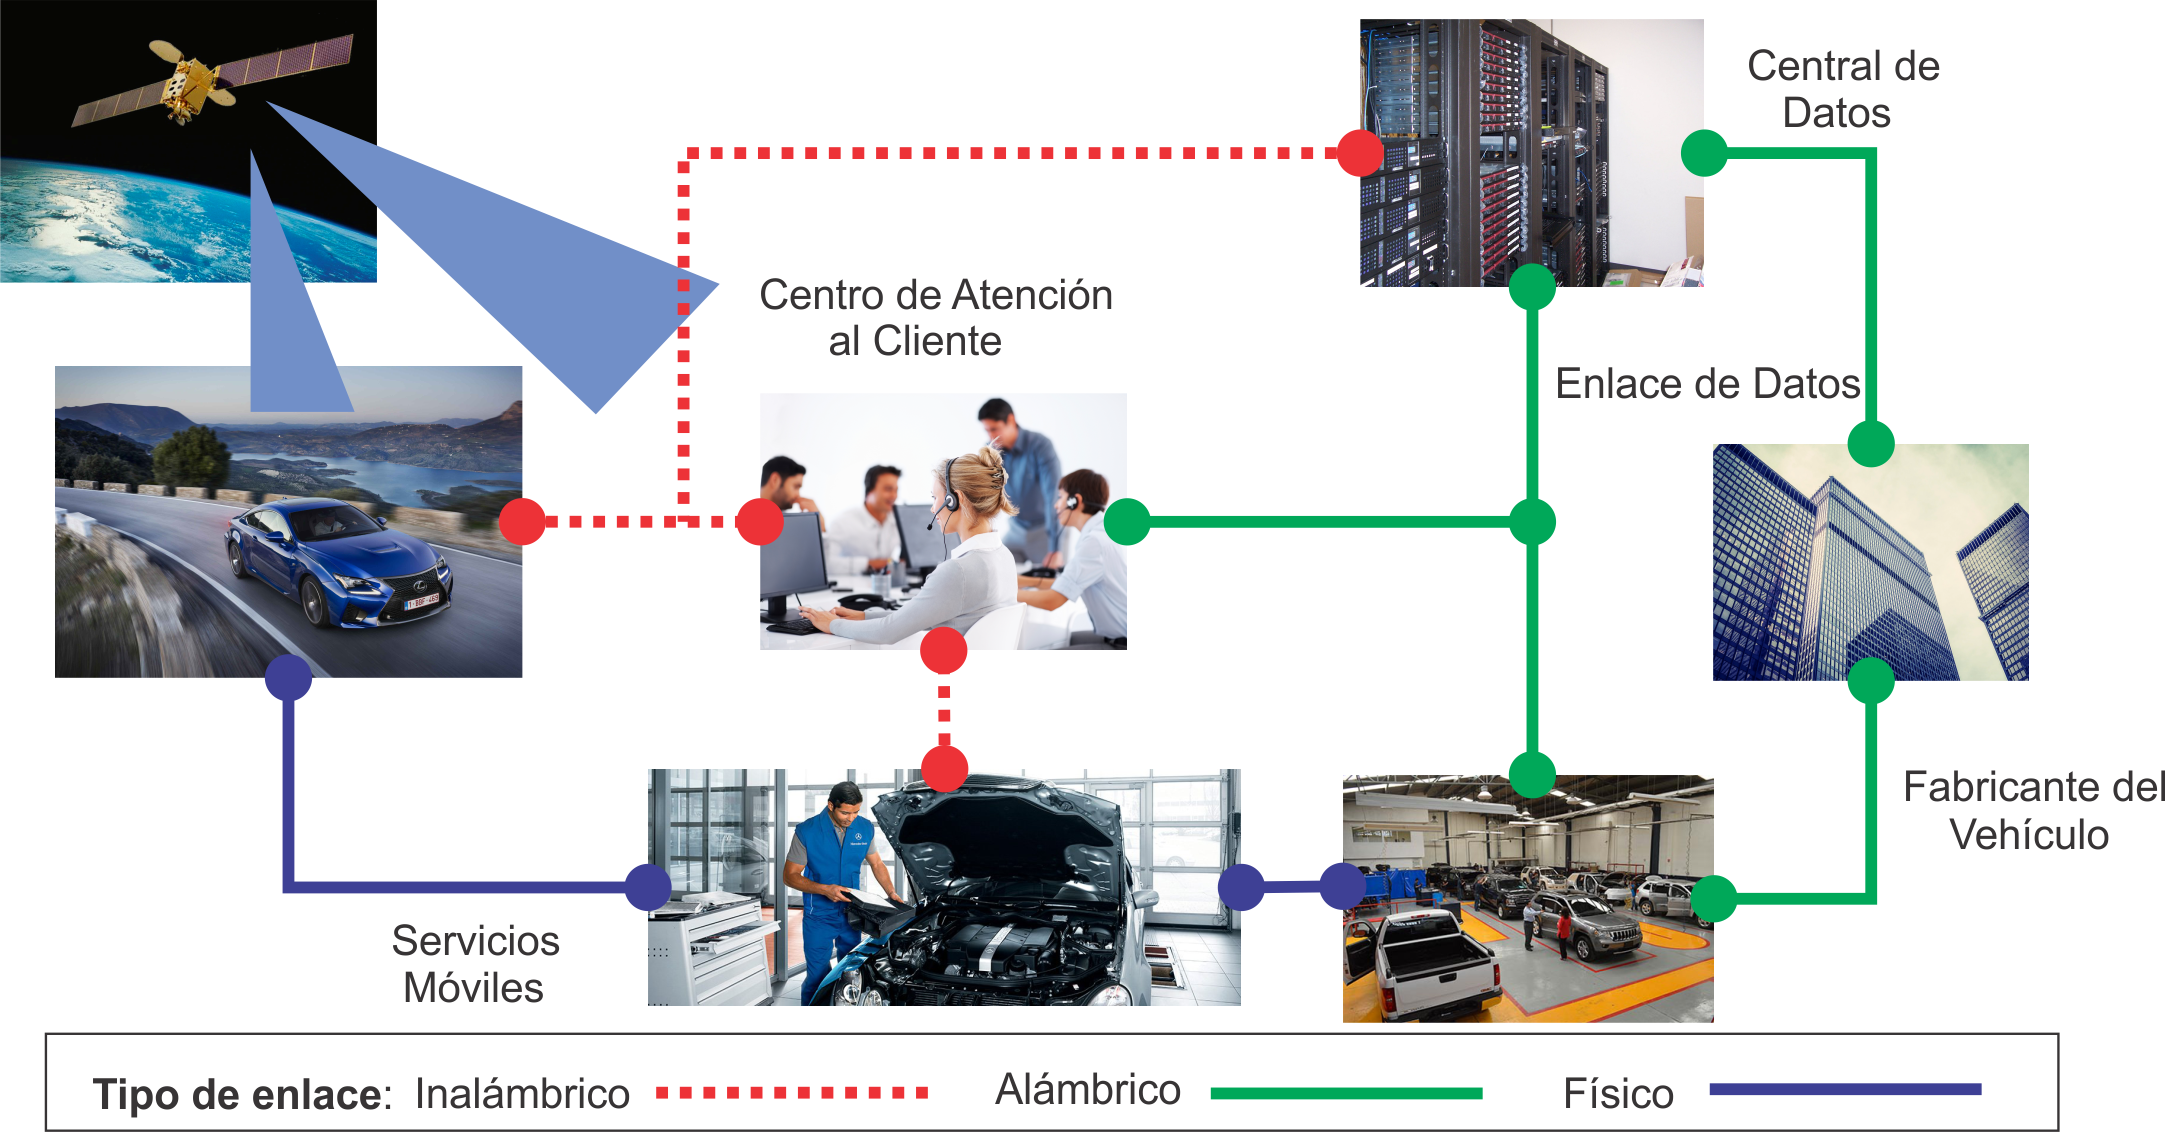
\includegraphics[width=0.8\textwidth]{./Cap2imagen/J_concepto_OBDIII.png}
	\caption[Diagrama de bloques general del concepto OBD-III.]{Diagrama de bloques general del concepto OBD-III.\textbf{ Fuente:} \cite{DE}.}
	\label{DenB} % preguntar que va aquí
\end{figure}


\section {EL Protocolo BUS CAN}

El desarrollo del  protocolo BUS CAN se debió al incremento de los dispositivos electrónicos en los vehículos como por ejemplo el administrador del motor, controlador de luces, aire acondicionado, entre otros.  El desarrollo del protocolo BUS CAN fue necesario para intercambiar de una mejor manera la información entre los diferentes sistemas de control y sus sensores.
Cuando no existía el protocolo BUS CAN los vehículos tenían un sistema de control e intercambio de información mediante conexiones punto a punto, es decir, los modulos que deseaban comunicarse entre si, debían estar conectados de forma directa o indirecta.
En una conexión  directa  cada línea de comunicación está asociada a un par de estaciones o dispositivos, los cuales intercambian información a través de dicha conexión, en cambio, en una conexión indirecta  la comunicación es realizada  mediante una o más estaciones intermediarias.
A medida que las necesidades de control en los vehículos  aumentaron se necesitaban de muchas conexiones y muchas líneas de comunicación, afectando considerablemente el costo de los materiales y el tiempo de producción del vehículo. La solución a este problema es la conexión de los dispositivos y sensores en un bus serial común para todos.

\subsection {Reseña Histórica}
La firma alemana Robert Bosch GmbH inició un proyecto de desarrollo de un protocolo de comunicación entre los distintos dispositivos y sensores  electrónicos para el interior del vehículo en el año 1983. Durante la especificación del sistema de bus serial se unió la empresa fabricante de automóviles Mercedez-Benz y el fabricante de semiconductores Intel Corp. 
Robert Bosch presenta oficialmente el sistema serial BUS CAN en febrero del año 1986, en el congreso de la Sociedad de Ingenieros Automotrices (SAE), celebrado en la ciudad de Detroit, Estados Unidos.
A un año después, la firma Intel realizo la primera implementación física del protocolo en el controlador CAN 82526 y tiempo después la firma Philips introdujo el controlador CAN 82C200, ambos integrados son la base del desarrollo de los controladores actuales.
No tardo mucho para que el protocolo BUS CAN trascendiera a ambientes fuera de lo automovilístico, de hecho las primeras aplicaciones aparecieron en las ramas industriales, como por ejemplo sistemas de control de elevadores, maquinas textiles, maquinas de rayos X entre otros.
Fue en 1992 cuando Mercedez-Benz implementó el protocolo  CAN en sus vehículos Clase "S". El sistema estaba compuesto por dos redes CAN, en la cual una red era de alta velocidad para la comunicación de las ECUs del motor, de la caja de cambios y el tablero de instrumentos; y una red de baja velocidad para el control del aire acondicionado y de los dispositivos electrónicos internos.  Esta implementación de Mercedez-Benz impulso a que otros fabricantes de automóviles comenzaran a utilizar redes BUS CAN en sus modelos de lujo, por ejemplo, BMW, Jaguar, Volvo, Saab, y VW, más tarde se agregaron a la lista Fiat, Renault y PSA. 
La estandarización del protocolo CAN se logro en el año 1993 bajo la norma ISO 11898. Varias versiones y mejoras aparecieron a partir de entonces, \cite{DSEEPC}.

\subsection {Clasificación de las Aplicaciones Automotrices}
La SAE estableció la siguiente clasificación formal de acuerdo a las áreas de aplicación dentro del automóvil:
\begin {itemize} 

\item \textbf{Clase A:} Se refiere a la comunicación con nodos no inteligentes como interruptores, luces, posición del asiento, posición de los espejos, seguros de puertas, etc. La información que se transmite requiere bajas velocidades de transferencia de datos, menor a 10Kbps. La conexión de cables es sencilla y los costos por conexión de nodos es bajo.

\item \textbf {Clase B:} En esta clase se distribuye una mayor cantidad de información, aquí se incluye la actualización del tablero de instrumentos y el control del aire acondicionado. La velocidad de transferencia de datos esta en el orden de 40Kbps

\item \textbf{Clase C:} Comprende la transmisión de datos en tiempo real (real time) con latencia de mensajes menores a 1ms. En esta clase los paquetes de datos transmitidos son mayor a 1 byte a una velocidad que va de 250Kbps a 1Mbps. Dentro de esta categoría están las aplicaciones de comunicación entre los diferentes sistemas de control  de motor, transmisión, estabilidad, frenos y dirección.

\item \textbf{Clase D:} En esta categoría se comunican grandes bloques de datos para aplicaciones de conexión del sistema de radio, teléfono, navegación GPS, consola de interfaz para controladores genéricos que tienen la finalidad de descargar programas, etc. La velocidad de datos requeridas está en el rango de 1 a 10Mbps \cite{DSEEPC}.
\end{itemize}

\section {Características del Protocolo BUS CAN}

El BUS CAN es un protocolo de comunicación serie que soporta control distribuido en tiempo real con un alto nivel de seguridad y multiplicación  \cite{PSMR}. La red de BUS CAN comunica todos los dispositivos a través de un único bus de comunicación de datos, a estos dispositivos se los denomina comúnmente como nodos. Cada nodo es capaz de interactuar con cualquier otro nodo sin la necesidad de una conexión punto a punto entre ellos.
El protocolo BUS CAN está definido internacionalmente por el conjunto de estándares ISO 11898, en dónde se definen las caracteristicas del protocolo, la capa física del bus, sus sistemas para alta y baja velocidad entre otros. El otro estándar que lo acompaña en el proceso de desarrollo del BUS CAN es la ISO 16845, el cual proporciona una  metodología y un conjunto de pruebas necesarias para comprobar la conformidad de cualquier implementación BUS CAN con base a la norma ISO 11898-1 \cite{ISO}, de esta manera se garantiza la comunicación entre los nodos BUS CAN de distintos fabricantes.

\subsection {Capas del Modelo OSI y Capas del Protocolo CAN}
El modelo de comunicación desarrollado por la ISO (International Organization for Standardization, por sus siglas en inglés), llamado OSI (Open System Interconnection, por sus siglas en inglés), es popular debido a que ayuda a dar una explicación  sencilla de la relación entre el hardware  y los protocolos utilizados en una red. El modelo OSI está conformado por 7 capas en las cuales cada una de las capas cumple con una función específica, que permite realizar la comunicación en una red.
La arquitectura del protocolo BUS CAN como muestra en la \textbf{Figura \ref{ABC}}, de acuerdo al modelo de referencia OSI incluye tres capas: Física, Enlace de Datos y Aplicación, además establece una capa especial para la gestión y control del nodo llamada Capa de Supervisor. 


\begin{figure}[H]
	\centering
		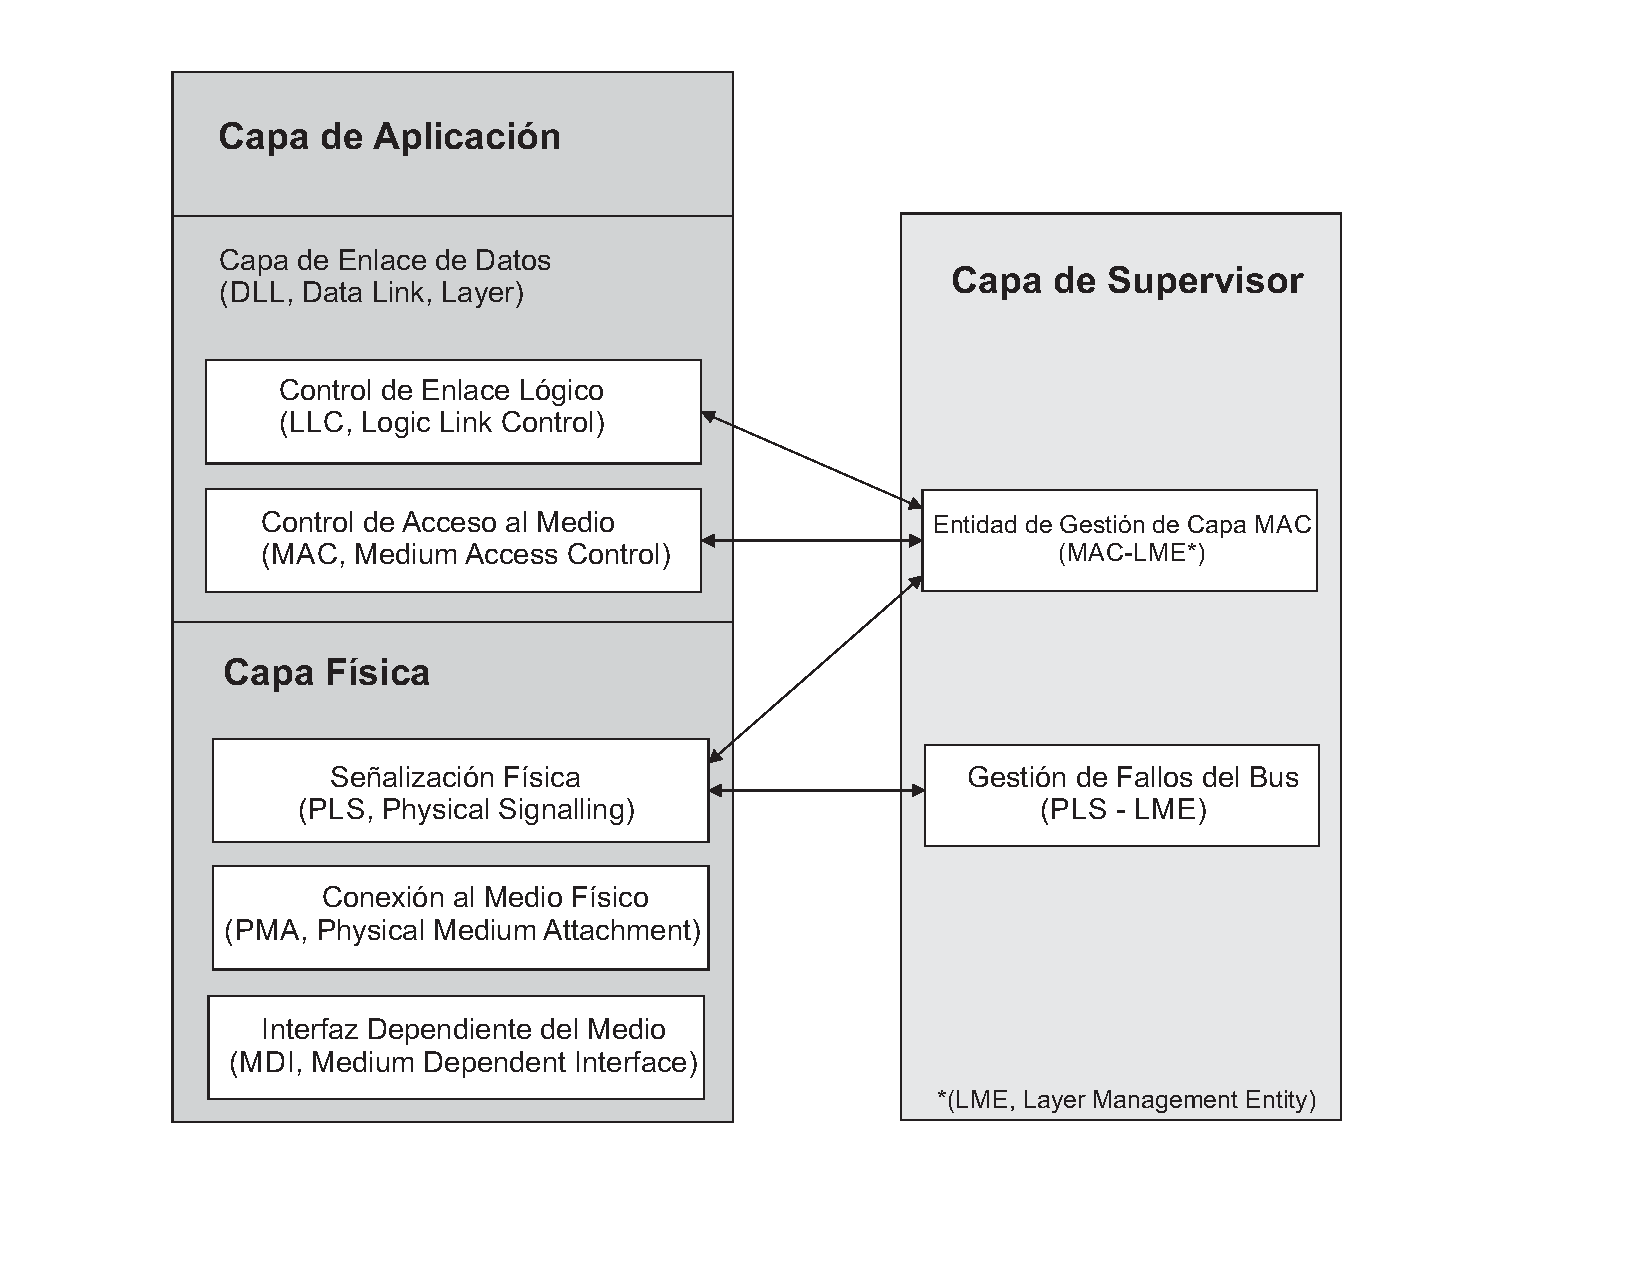
\includegraphics[width=0.8\textwidth]{./Cap2imagen/protocolocan.pdf}
	\caption[Arquitectura de protocolos BUS CAN.]{Arquitectura de protocolos BUS CAN.\textbf{ Fuente:} \cite{DSEEPC}.}
	\label{ABC} % preguntar que va aquí
\end{figure}

\subsubsection  {Capa Física}

La capa física es responsable por la transferencia de bits entre diferentes nodos de red y define los aspectos del medio físico para la transmisión de datos entre los nodos. Los más importantes hacen referencia a los niveles de señal, sincronización, representación y tiempos en que los bits se transfieren al bus. 
Las especificaciones Bosch del protocolo BUS CAN no define una capa física, sin embargo, el estándar  ISO 11898 establece las características que deben cumplir las aplicaciones para la transferencia en alta y baja velocidad.
 
%\subsubsubsection{SubCapa Fisica} %%%%%% lo cambie
\paragraph{SubCapa Física}

La SubCapa de señalización física (PLS, Physical Layer Signalling, por sus siglas en inglés) define la representación, tiempo y sincronización de los bits, y está implementada en los controladores del protocolo BUS CAN.


%\subsubsubsubsection {Representación de los bits}
\paragraph{Representación de los Bits}

Una trama BUS CAN está codificada de acuerdo con el método NRZ (No Return Zero, por sus siglas en inglés), el cual produce una frecuencia de menor operación. Sin embargo, en el caso de transmitir una gran cantidad de bits con la misma polaridad, la codificación NRZ no proporciona flancos que puedan utilizarse en la sincronización y para ello se implementa el procedimiento de inserción de bit (bit-stuffing) \textbf{Figura \ref{IB}}, Asegura que en la transmisión de una trama BUS CAN solamente puede haber un máximo de 5 bits consecutivos con la misma polaridad.



\begin{figure}[H]
	\centering
		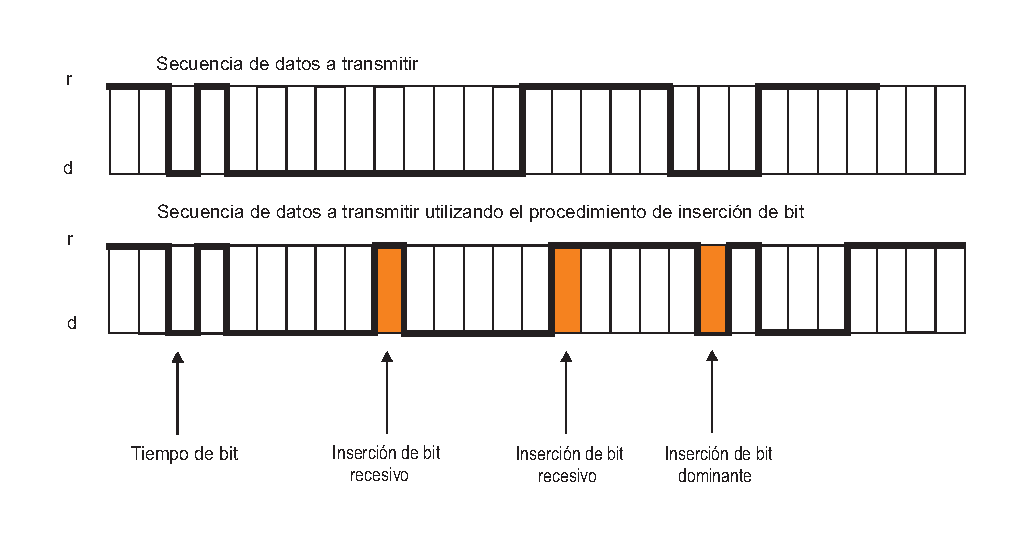
\includegraphics[width=0.8\textwidth]{./Cap2imagen/insercionbit.pdf}
	\caption[Inserción de bit.]{Inserción de bit.\textbf{ Fuente:} \cite{DSEEPC}.}
	\label{IB} % preguntar que va aquí
\end{figure}

%\subsubsubsubsection {Temporización de Bits}
\paragraph{Temporización de Bits}

 El protocolo BUS CAN tiene flexibilidad para determinar los parámetros de velocidad de transferencia, punto de muestreo de bit y número de muestras realizadas en un periodo de bit. Por lo tanto en el diseño de una red BUS CAN se debe tener en cuenta los siguientes conceptos:

\begin{itemize}

\item Tiempo de bit ($t_b$): es el tiempo de duración de un bit.
\item Velocidad de transferencia nominal ($f_b$): es el número de bits por segundo que una transmisión ideal emite sin sincronización.
\item Tiempo de bit nominal: se obtiene mediante la \textbf{Ecuación \ref{eq1}} y se divide en cuatro segmentos de tiempo.

\end{itemize}

La longitud de los segmentos de tiempo en un intervalo de bit está definida en multiples enteros definidas por el periodo de un  oscilador $t_{clk}$. El parámetro $t_q$ es la unidad de tiempo discreta más pequeña utilizada en un modulo BUS CAN. En la \textbf{Figura \ref{TB}} se puede observar los segmentos de tiempo de un bit y en la \textbf{Figura \ref{DB}} se puede observar la derivación del tiempo de un bit.

%insertar ecuacion:::
\begin {equation}
\label {eq1}
t_b = \frac {1}{f_b}
\end {equation}
% insertar ecuacion___

\begin{figure}[H]
	\centering
		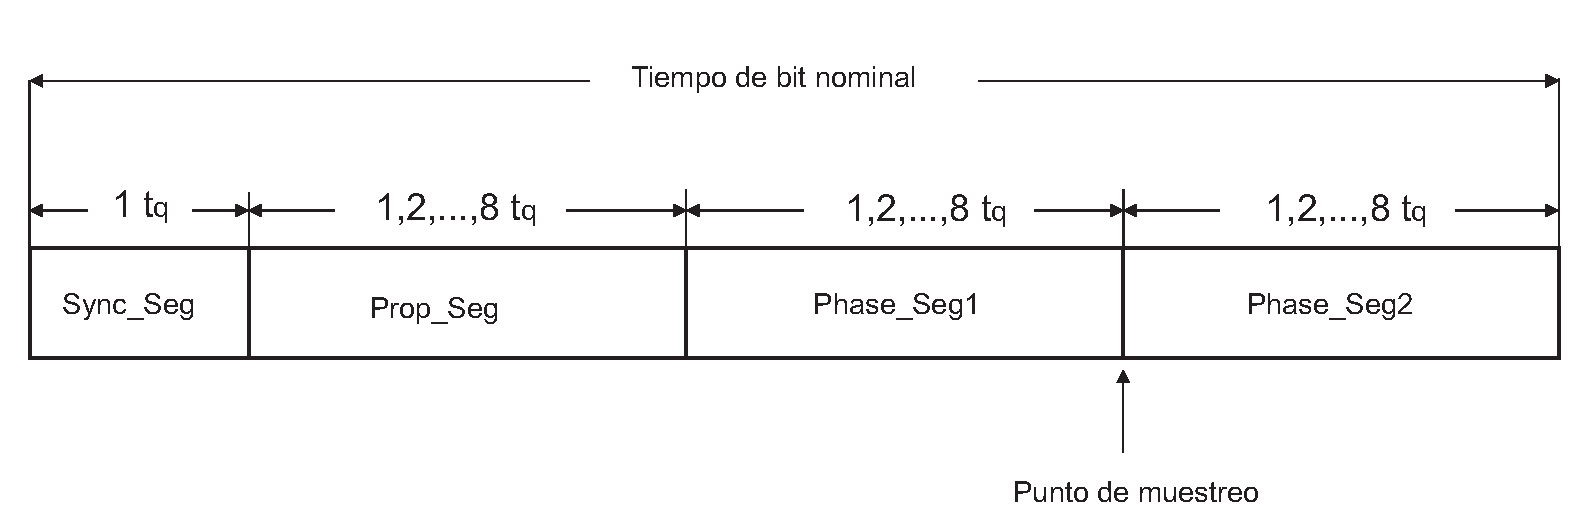
\includegraphics[width=0.8\textwidth]{./Cap2imagen/tiempo_bit.pdf}
	\caption[Segmento del tiempo de un bit.]{Segmento del tiempo de un bit.\textbf{ Fuente:} \cite{DSEEPC}.}
	\label{TB} % preguntar que va aquí
\end{figure}

\begin{figure}[H]
	\centering
		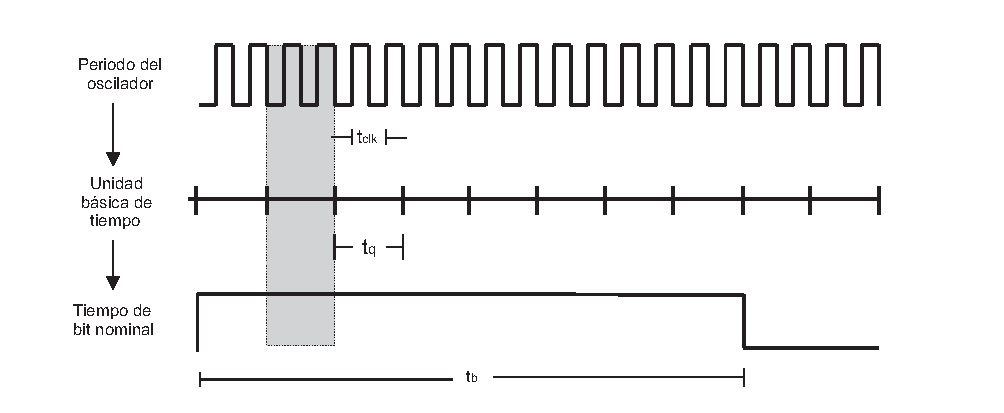
\includegraphics[width=0.8\textwidth]{./Cap2imagen/derivacion_bit.pdf}
	\caption[Derivación del tiempo de un bit.]{Derivación del tiempo de un bit.\textbf{ Fuente:} \cite{DSEEPC}.}
	\label{DB} % preguntar que va aquí
\end{figure}


Los cuatro segmentos que forman un tiempo de bit nominal son:

\begin{itemize} % para crear una lista
\item Segmento de sincronización (Sync Seg): se utiliza para sincronizar los diferentes nodos del bus en un flanco dentro del mismo segmento.
\item Segmento de tiempo de propagación (Prog Seg): sirve para compensar los tiempos de retardos físicos originados por la propagación de la señal en el bus y por los retardos internos en los nodos.
\item Segmento de memoria temporal de fase 1 (Phase Seg1): se utiliza para compensar variaciones de tiempo entre los nodos y puede incrementarse durante la resincronización.
\item Segmento de memoria temporal de fase 2 (Phase seg2): se utiliza para compensar variaciones de tiempo entre los nodos y puede reducirse durante la resincronización.

\item Punto de muestreo (sample point): instante del tiempo en que se lee e interpreta el nivel del bus y se proporciona el valor del bit respectivo.
\item Tiempo de procesamiento de la información: Es el periodo de tiempo que comienza con el punto de muestreo y se utiliza para calcular el nivel de bit subsecuente.
\end{itemize}

Para la transferencia de bits entre distintos nodos de red es necesario estudiar la capa física, la cual define parámetros como los niveles de señal, la sincronización, la impedancia de la línea de bus de comunicación de acuerdo con el medio físico adoptado y la velocidad de comunicación entre ellos. En el protocolo BUS CAN no todos los nodos conectados a la red mediante el bus necesitan transmitir a la misma velocidad, esto dependerá de las funciones que desempeña cada nodo y de la importancia de sus mensajes, es por ello que el protocolo BUS CAN posee varias tasas de transmisión de bits especificados  por el estándar ISO. Las velocidades van desde la tasa baja de 125kbps hasta la tasa alta de 1Mbps.
La capa física define el medio de transmisión. La representación de los niveles lógicos en las líneas del bus de comunicación BUS CAN es realizada de acuerdo al nivel de tensión que serán establecidos en el mismo bus. Existen dos variables para representar las líneas del BUS: CANH y CANL. Un bit recesivo (1 lógico) es representado a través de dos líneas del bus con un nivel de tensión de 2.5V, de modo que la diferencia de potencial entre CANH  y CANL será de 0V, en cambio, un bit dominante (0 lógico) es representado colocando el CANH = 3.5V y el CANL = 1.5V. Esto da una diferencia de potencial para un bit dominante de cerca de 2V, \cite{PSMR}. De esta manera los datos no son representados por bits de nivel “0” y “1”, sino son representados por bits dominantes y recesivos como se muestra en la \textbf{Figura \ref{N_N}} . 


\begin{figure}[H]
	\centering
		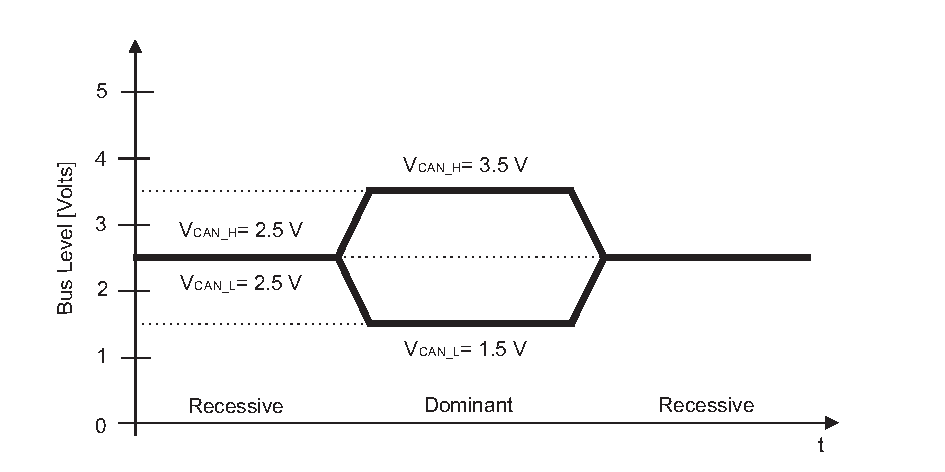
\includegraphics[width=0.8\textwidth]{./Cap2imagen/niveles.pdf}
	\caption[Niveles nominales de la señal BUS CAN ISO 11898.]{Niveles nominales de la señal BUS CAN ISO11898.\textbf{ Fuente:} \cite{PSMR}.}
	\label{N_N} % preguntar que va aquí
\end{figure}

Para evitar que los datos sean reflejados en forma de eco en el BUS de comunicación se colocan en los extremos del BUS, entre CANH y CANL, unas resistencias cuyos valores son empíricos, como se muestra en la \textbf{Figura \ref{T_B}}. 


\begin{figure}[H]
	\centering
		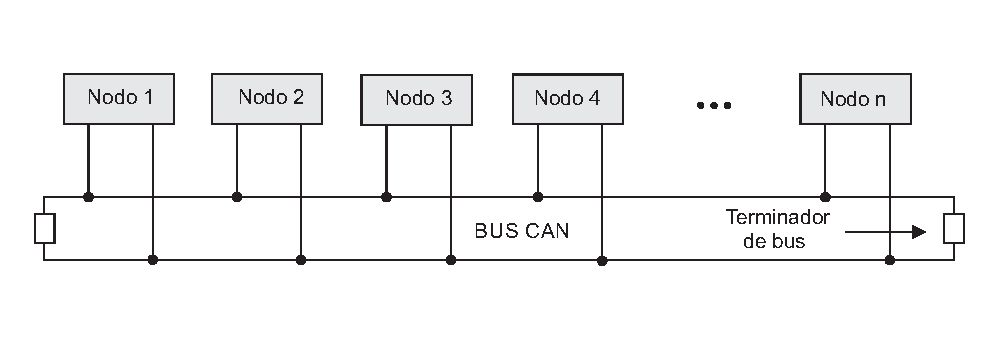
\includegraphics[width=0.8\textwidth]{./Cap2imagen/terminador.pdf}
	\caption[Terminador de bus.]{Terminador de bus.\textbf{ Fuente:} \cite{PSMR}.}
	\label{T_B} % preguntar que va aquí
\end{figure}


\subsubsection {Capa de Enlace de Datos}
%%%% desde aqui
Esta capa describe el método para el intercambio de datos entre nodos dentro de un medio común.
Los mensajes transmitidos por la red BUS CAN tiene dos versiones: la 2.0A y la 2.0B, en la primera un campo de la trama, destinado para el identificador,  está formada por 11 bits mientras que en la segunda está formada por 29bits.
En la capa de enlace para el protocolo BUS CAN se utilizan dos subcapas: MAC (Media Access Control) y LLC (Logical Link Control).

\subsubsection {MAC}

En la red BUS CAN se brinda procesamiento en tiempo real a todos los nodos conectados al bus.  Para que los nodos tengan acceso al medio se utiliza un mecanismo de arbitraje que se describe a continuación:

\begin{itemize}
\item Cuando un nodo intenta acceder al medio y comunicarse con otro nodo, la capa de aplicación realiza la petición para envío de trama. En esta situación puede ocurrir que la capa de aplicación de varios nodos inicien el mismo procedimiento simultáneamente. Esto en el protocolo BUS CAN se resuelve asignando prioridades mediante el ID (identificador) de cada mensaje \textbf{Figura \ref{LID}}. Esto se realiza en el diseño del sistema, no puede modificarse de forma dinámica. El ID con menor número binario es el que posee mayor prioridad.
\item Para acceder al medio se utiliza el CSMA/CD+AMP (Carrier Sense Multiple Access/Collision Detection with Arbitration on Message Priority, por sus siglas en inglés). Esto hace que los nodos que desean transmitir un mensaje en la red deban esperar a que el bus este libre, cuando esto pasa los nodos transmiten un bit de inicio (acceso multiple). Cada nodo lee el bus durante la transmisión y compara bit a bit la trama transmitida con la recibida, si se detecta una diferencia se lleva a cabo un mecanismo de arbitraje.

\end {itemize}

\begin{figure}[H]
	\centering
		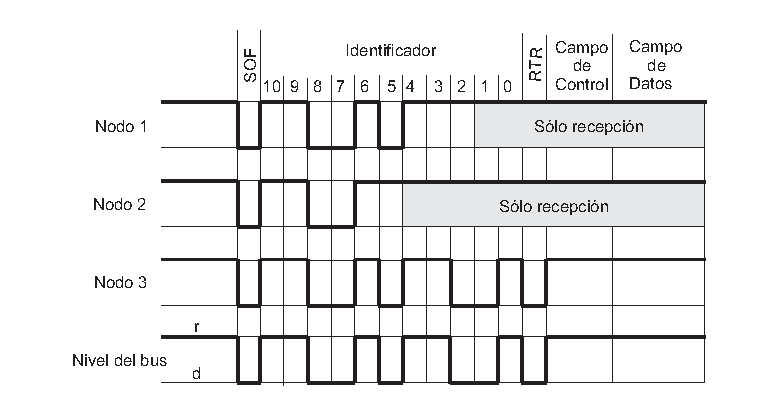
\includegraphics[width=0.8\textwidth]{./Cap2imagen/logicacan.pdf}
	\caption[Lógica del BUS CAN.]{Lógica del BUS CAN.\textbf{ Fuente:} \cite{PSMR}.}
	\label{LID} % preguntar que va aquí
\end{figure}


\subsubsection {LLC}
Es la capa del enlace de datos cuyas funciones son:

\begin {itemize}
\item Filtrar mensajes: El ID no define la dirección de destino del mensaje pero si el contenido, cada receptor recibe el mensaje y el mismo receptor determina si es para él o no.
\item Notificar sobrecarga: si las condiciones internas del receptor requieren un retraso en la transmisión del mensaje, la sub capa LLC transmite una notificación de sobre carga.
\item Proceso de recuperación: La sub capa LLC da la posibilidad de retransmisión automática de tramas cuando pierde su arbitraje o presenta un error en la transmisión.
\end{itemize}

\subsubsection {Transmisión de Mensajes}
Para la transmisión y control de mensajes se define cuatro tipos de tramas: la trama de datos, la trama remota , la trama de error y la trama de sobre carga.

\begin{itemize} % ITEM PRINCIPAL
\item Trama de datos:  la trama de datos está formada por 7 campos, \textbf{Figura: \ref{TRD}}.

			\begin{figure}[H]
			\centering
				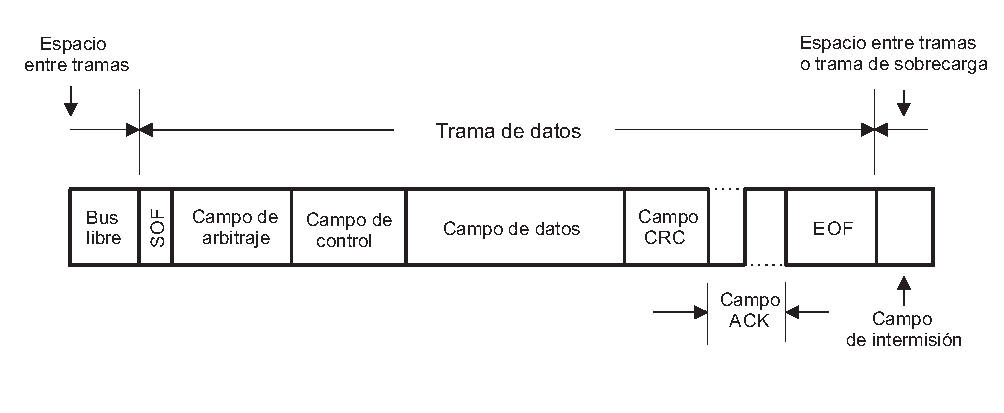
\includegraphics[width=0.9\textwidth]{./Cap2imagen/trama_datos.pdf}
			\caption[Formato de la trama de datos.]{Formato de la trama de datos.\textbf{ Fuente:} \cite{PSMR}.}
			\label{TRD} 
			\end{figure}

				\begin{itemize} %ITEM SECUNDARIO%4tabulaciones
				\item SoF (Stad of Frame): determina el inicio de la trama de datos y consiste en un bit dominante que sincroniza a todos los nodos activos en la red. Es el mismo para la trama estándar y extendida del BUS CAN.
				\item Arbitration field: este campo cambia de acuerdo al formato de la trama.
										
											\begin {itemize} %ITEM TERCIARIO%8tabulaciones
											\item El formato estándar está formado por un identificador de $11$ bits  y el bit de petición de transmisión remota RTR (Remote Transmission Request, por sus siglas en inglés). El bit menos significativo del identificador se transmite al último, además, no pueden ser recesivos los 7 bits más significativos.
											\item En el formato extendido la trama tiene un identificador de $29$ bits, el bit de petición substituta SRR(Sustitute Remote Request, por sus siglas en inglés), el bit de extensión del identificador IDE(Identifier Extension) y el bit RTR. El identificador se divide en dos secciones: la primera denominada base (base ID) que es de $11$bits y la segunda sección de 18 bits conocida como extendida (extended ID). Los bits se transmiten en orden de mayor a menor prioridad.
											\end {itemize} % FIN DE TERCIARIO

El bit RTR debe ser dominante para ambos formatos de trama de datos y el bit SRR es un bit recesivo, por lo tanto las posibles colisiones entre ambos tipos de formatos de trama que tengan el mismo valor en el campo Base ID se resuelven de manera que el formato de trama estándar predomina sobre el formato de trama extendida. En dicha resolución también se involucra el bit IDE, el cual pertenece al campo de arbitraje en el caso de un formato extendido y se encuentra en el campo de control para el caso de un formato de trama estándar. La transmisión del bit IDE es dominante para el formato estándar y recesivo para el extendido. En la \textbf{Figura: \ref{FEE}} se especifica la diferencia entre el formanto estándar y el formato extendido

			\begin{figure}[H]
			\centering
				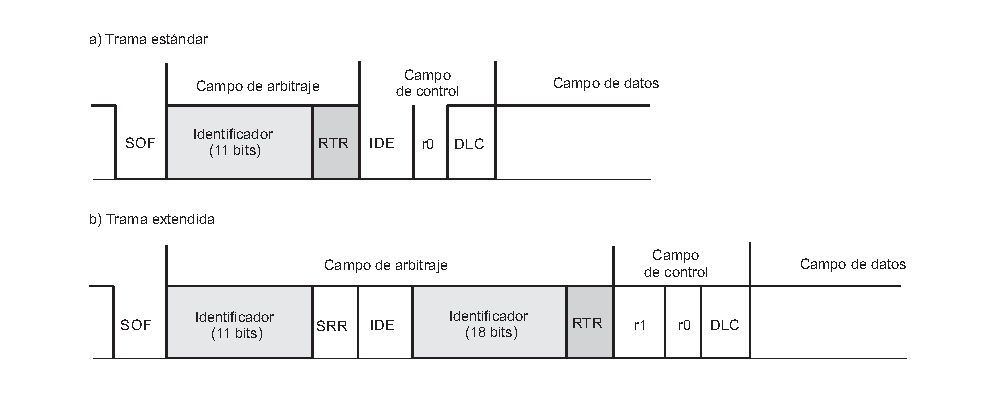
\includegraphics[width=0.9\textwidth]{./Cap2imagen/datos_est_ext.pdf}
			\caption[Trama de datos estándar y extendido.]{Trama de datos estándar y extendido.\textbf{ Fuente:} \cite{PSMR}.}
			\label{FEE} 
			\end{figure}


				
				
				\item Control Field: Está compuesto de seis bits, IDE/r$1$, r$0$ y cuatro bits que forman el código de longitud de datos DLC (Data Length Code, por sus siglas en inglés). El primer bit que se transmite es IDE, el cual distingue entre los dos tipos de tramas; seguida r$0$, en nivel dominante y está reservado para futuras aplicaciones del protocolo BUS CAN; finalmente se transmite el DLC para indicar el numero de octetos contenidos en el campo de datos. 
				\item Data Field: Puede tener una longitud de $0$ a $8$ octetos y contiene el mensaje a transmitir en la trama de BUS CAN. EL bit con mayor prioridad se transfiere primero.
				\item CRC (Cyclic Redundant Check, por sus siglas en inglés): Es una secuencia de $15$ bits de verificación y un bit delimitador CRC (CRC delimiter) transmitido en un nivel recesivo. Mediante este campo se verifica si la trama fue alterada.
				\item ACK (Acknowledgement, por sus siglas en inglés): está formada por dos bits : ACK (ACK slot) y delimitador ACK (ACK delimiter), este último siempre se transmite en un nivel recesivo. Todo nodo activo en la red CAN que recibe una trama válida, sobrescribe la ranura ACK con un nivel dominante, y con ello el transmisor verifica que su mensaje se envió correctamente. si por el contrario ningún nodo sobrescribe dicha ranura, el transmisor considera un error de transmisión.
				\item End of Frame: El fin de la trama de datos y la trama remota están delimitadas por una secuencia de 7 bits recesivos que indican el fin de la trama. Cuando el EOF está activo se realiza una violación al procedimiento de inserción de bit, por ello dicho procedimiento no se aplica a este campo.
				\end{itemize} %FIN SECUNDARIO



\item Trama remota: permite iniciar una transmisión de mensaje de un nodo estando este en modo recepción mediante el envío de esta trama. Los campos de una trama remota son los mismos que la de una trama de datos, a excepción que la trama remota no contiene el campo de datos y el bit RTR es recesivo. EL valor del DLC debe coincidir con el de la trama de datos correspondiente. En la \textbf{Figura: \ref{TR}} se exponen las características de la trama.

			\begin{figure}[H]
			\centering
				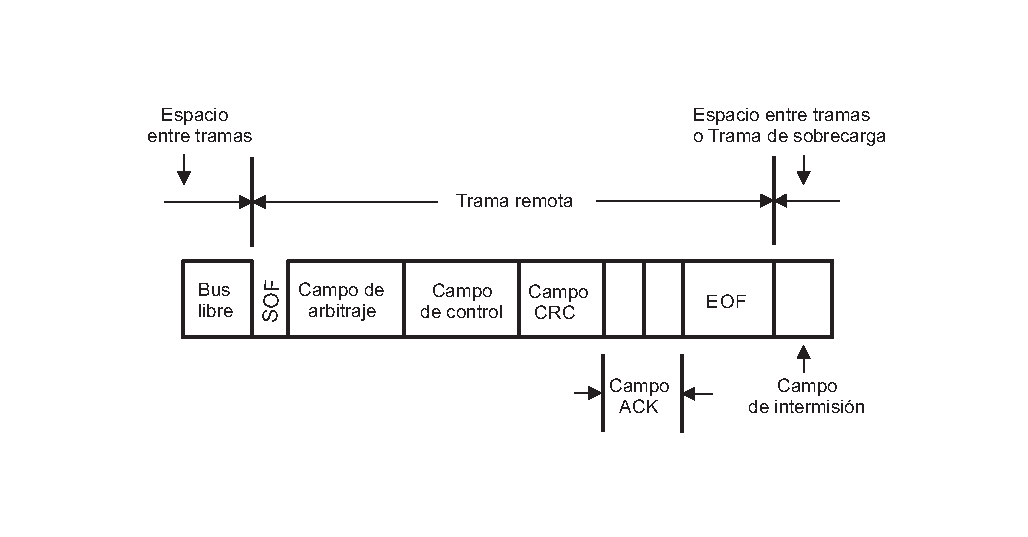
\includegraphics[width=0.9\textwidth]{./Cap2imagen/tramaremota.pdf}
			\caption[Formato de trama remota.]{Formato de trama remota.\textbf{ Fuente:} \cite{DSEEPC}.}
			\label{TR} 
			\end{figure}


\item Trama de error: durante la transmisión o recepción de una trama de datos o una trama remota, esta trama señaliza la detección de un error, iniciando nuevamente el envió del mensaje. En la \textbf{Figura: \ref{TE}} se expone como la trama de error está formada por dos campos:

							\begin{itemize}
							\item Error flag: hay dos formas de representarla:
										\begin {itemize}
										\item Active error flag: son seis bits dominantes consecutivos.
										\item Passive error flag: son seis bits recesivos consecutivos, pero pueden sobrescribirse con bits dominantes de otros nodos.
										\end {itemize}
							\item Error delimiter: una trama de error termina con una secuencia de $8$ bits recesivos. Posterior a la transmisión de una bandera de error, el nodo transmite bits recesivos y verifica el nivel del bus hasta que reconozca un bit recesivo, entonces comienza la transmisión de otros siete bits recesivos. Con este mecanismo, el nodo puede determinar si fue el primero en transmitir una bandera de error y con ello detectar una condición de error.
							\end {itemize}
							
								\begin{figure}[H]
								\centering
								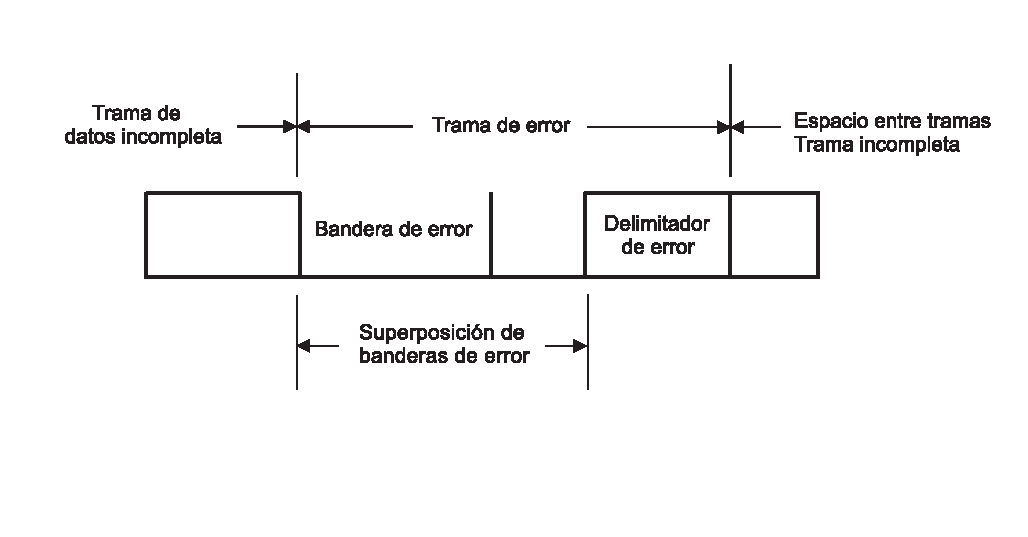
\includegraphics[width=0.9\textwidth]{./Cap2imagen/trama_error.pdf}
								\caption[Formato de trama de error.]{Formato de trama de error.\textbf{ Fuente:} \cite{DSEEPC}.}
								\label{TE} 
								\end{figure}


					
\item Trama de sobre carga: un receptor puede solicitar un retraso en la transmisión de la siguiente trama si las condiciones internas del receptor requieren un retraso en la transmisión del mensaje. Se permite en el protocolo BUS CAN el envio de dos tramas de sobre  carga como máximo, \textbf{Figura: \ref{TSC}}.
Las tramas de sobrecarga se transmiten después de detectar las siguientes condiciones de error: 


					\begin{itemize}
		
					\item Detección de un bit dominante durante los primeros dos bits del campo de intermisión. La detección de un bit dominante en el tercer bit del campo de intermisión se interpreta como un SOF. 
					\item Cuando un receptor detecta un bit dominante en el ultimo bit del campo EOF, o cuando un nodo receptor o transmisor detecta un bit dominante en el ultimo bit del delimitador de una trama de error o sobrecarga.
					\end{itemize}

Una trama de sobrecarga se considera una forma especial de trama de error y tiene los siguientes campos:
	
								\begin{itemize}
								\item Overload flag: se constituye por ocho bits dominantes. La forma completa corresponde a la bandera de error activa.
								\item Oveload delimiter: formado por 8 bits recesivos.
								\end{itemize}


			\begin{figure}[H]
			\centering
				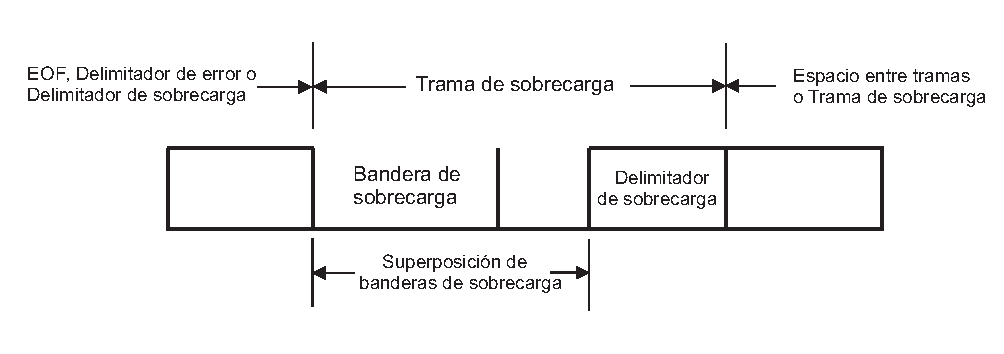
\includegraphics[width=0.9\textwidth]{./Cap2imagen/sobrecarga.pdf}
			\caption[Formato de trama de sobrecarga.]{Formato de trama de sobrecarga.\textbf{ Fuente:} \cite{DSEEPC}.}
			\label{TSC} 
			\end{figure}
				
\end{itemize}

\subsubsection {Espacio Entre Tramas}

Para tener en cuenta las tramas de datos y las tramas remotas están separadas por un espacio entre tramas, en cambio las tramas de error y las tramas de sobrecarga se transmiten en forma sucesiva.
Además el espacio entre tramas está formado por tres campos:

	\begin{itemize}
	\item Intermission: Consiste en tres bits recesivos. Durante su transmisión la única acción que puede realizarse es señalar una condición de sobrecarga, y no se permite que ningún nodo inicie la transmisión de una trama de datos o remota. 
	\item Bus Idle: Se mantiene un nivel recesivo hasta que un nodo inicie la transmisión de una trama nueva.
	\item Suspend transmission: El espacio entre tramas contiene un tiempo de inhibición de transmisión de ocho bits para nodos que se encuentran en estado de error pasivo.
	\end{itemize}


%\subsubsubsubsection {Codificación de Tramas}
\paragraph{Codificación de Tramas}

Los campos de inicio de trama, identificador, control, datos y CRC están codificados de acuerdo al procedimiento de inserción de bit. Los campos restantes como el delimitador CRC, ACK y EOF tienen un formato fijo y no siguen el procedimiento de inserción de bit, de igual forma, las tramas de error y sobrecarga tienen un formato fijo y no se codifican por dicho procedimiento.

%\subsubsubsubsection {Validación de Tramas}
\paragraph{Validación de Tramas}

Para validar un trama difiere según el:

\begin {itemize}
\item Transmisor: La trama es válida si no existen errores hasta el final del campo EOF. Si existe un error, en la trama se activa el proceso de recuperación.
\item Receptor: la trama es válida si no existen errores hasta el siguiente bit después del campo EOF.
\end{itemize}


%\subsubsubsubsection {Detección y Manejo de Errores}
\paragraph{Detección y Manejo de Errores}

En una red el controlador de BUS CAN tiene la capacidad de detectar y manejar errores que surjan en la comunicación. Si un nodo detecta un error inmediatamente lo comunica al resto de  los nodos de la red. Si algún nodo lanza errores continuamente el protocolo BUS CAN tiene un algoritmo que se basa en la actividad del bus para desconectar a los nodos que envían fallos permanentemente, de esta manera los demás nodos no son perturbados por estos nodos defectuosos.

%\subsubsubsubsection {Mecanismo de Detección de Errores}
\paragraph{Mecanismo de Detección de Errores}

Para mantener la seguridad de la transmisión de datos, el protocolo BUS CAN define los siguientes mecanismos para la detección de errores: 
\begin{itemize}
\item Monitoreo de bits: Todo nodo verifica que el nivel de bits transmitido sea el mismo nivel del bus, y cuando dichos valores difieren se detecta un bit de error. El monitoreo de bits representa un mecanismo de seguridad global para la detección de todos los errores efectivos.
\item Verificación del procedimiento de inserción de bit: hace referencia al hecho de detectar un error de inserción de bit cuando ocurren seis niveles consecutivos de bits con el mismo valor en un campo de trama codificado por el procedimiento de inserción de bit (Stuff error).
\item Verificación de redundancia cíclica de 15 bits: Se detecta un error de CRC cuando la secuencia de CRC calculada por el nodo no corresponde al campo CRC de la trama recibida.
\item Verificación de trama: Cuando un campo fijo contiene uno o más bits no válidos se detecta un error. 
\item Verificación de aceptación: un transmisor detecta un error de aceptación (ACK error) cuando el slot ACK no cambia de estado dominante.
\end{itemize}


%\subsubsubsubsection {Manejo de Errores}
\paragraph*{Manejo de Errores}

Cuando un nodo detecta algún tipo de error, ya sea de bit, de inserción, de forma o de aceptación, inicia una transmisión de un error flag en el siguiente bit. Cuando se detecta un error de CRC, se inicia la transmisión de una trama de error después del delimitador ACK, a excepción de que previamente se haya transmitido otra trama de error.
El manejo de errores se lleva acabo de acuerdo con el diagrama de flujo de la \textbf {Figura: \ref{D_F}}
%width = 0.33
\begin{figure}[H]
	\centering
		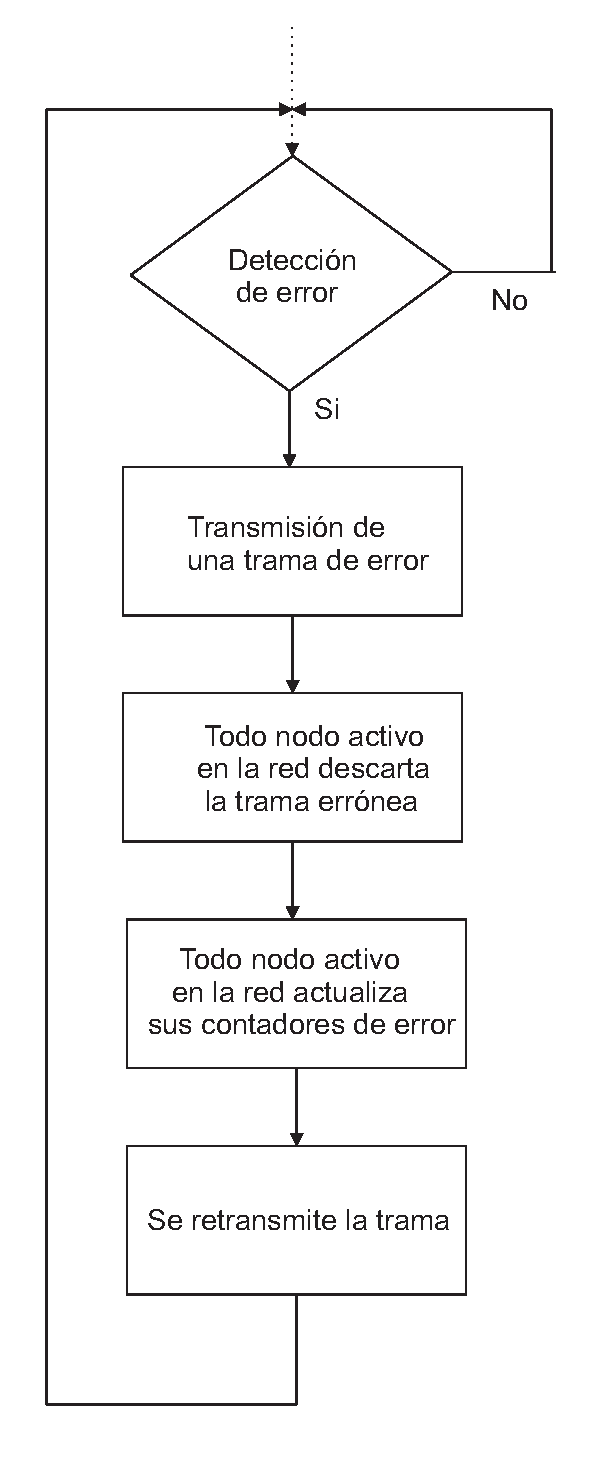
\includegraphics[width=0.40\textwidth]{./Cap2imagen/diagrama.pdf}
	\caption[Diagrama de flujo para manejar errores.]{Diagrama de flujo para manejar errores.\textbf{ Fuente:} \cite{DSEEPC}.}
	\label{D_F} % preguntar que va aquí
\end{figure}

%\subsubsubsubsection {Capacidad de Detección de Errores}
\paragraph{Capacidad de Detección de Errores}

Se utilizan diferentes mecanismos para detectar errores en los protocolos de bus seriales, generalmente se encarga el receptor de esta verificación. La capacidad de detectar errores de transmisión depende de los mecanismos de error y del protocolo utilizado.




\subsubsection {Capa de Aplicación}

La capa de Aplicación no se encuentra especificada en el estándar, por lo que se deja al usuario en la libertad de desarrollarla.
Existen varias aplicaciones utilizadas como por ejemplo CANopen, DeviceNet y CAN aerospace. 

Para utilizar una red BUS CAN de dos lineas, es recomendable utilizar el par trenzado para establecer la comunicación entre estos, debido a que este tipo de cable atenúa los efectos causados por interferencias electromagnéticas. 
La velocidad en una red  BUS CAN es inversamente proporcional a la longitud del bus de comunicación. La mayor tasa de bits especificada es de 1Mbps a una distancia entre nodos de 40m. 

\subsection {Hardware BUS CAN}

\subsubsection{Transceiver}

El Transceiver se encarga de adaptar las señales de un controlador CAN  a los niveles utilizados por el nivel físico. Actúa como transmisor y receptor de datos. Transforma los datos utilizados por el controlador BUS CAN en señales eléctricas que son compatibles con las características eléctricas del bus de comunicación. De la misma manera, este recibe los datos del bus de comunicación y los adapta para que pueda ser recibida por el controlador BUS CAN.

\subsubsection {Controlador BUS CAN}

Encargado de la comunicación entre el microprocesador de la unidad de control y el transceiver. 
 
\subsection{Estandares Existentes}

%Estandares <<
Para entender los estándares presentes en el mercado del protocolo BUS CAN se deben comprender el trabajo de las siguientes sociedades:

\textbf{ SAE Internacional (SAE - Society of Automotive Engineers)}: La Sociedad de Ingenieros Automoción, es la organización enfocada en la movilidad de los profesionales en la ingeniería aeroespacial, automoción, y todas las industrias comerciales especializadas en la construcción de los vehículos. El principal objetivo de la sociedad es el desarrollo de los estándares para todos los tipos de vehículos, incluyendo coches, camiones, barcos, aviones, etc. Cada uno que se interese por los factores humanos y los estándares ergonómicos, puede ser miembro de esta organización. 

Entre uno de los estándares encontramos al OBD-II, todos los vehículos modernos están equipados con el sistema diagnóstico conocido como On-Board Diagnostics II (OBDII, por sus siglas en inglés). Si este funciona mal, la luz de control del motor se enciende para avisar al conductor que tiene que revisar los códigos DTC (Diagnostic TRouble Codes):

SAE se encarga de la estandarización de los datos que se utilizan en el protocolo BUS CAN y en otros protocolos de comunicación en vehículos de automoción, es decir, para los automóviles terrestres estandariza el sistema de diagnóstico conocido como OBD II.

Los estándares SAE más conocidos son: 

\textbf{SAE J1962}: Define las características del conector OBD II.  La especificación prevé dos interfaces de hardware estándar, llamado conector tipo A y conector tipo B, de 16 pines. Ambos tipos tienen una ranura entre las dos filas de pines, pero el tipo B tiene la ranura interrumpida en el medio, \cite{J1962}. 

\textbf{SAE J1979}: Define un método para la solicitud de varios datos de diagnóstico y una lista de parámetros estándar que podrían estar disponibles a partir de la ECU (engine control unit, por sus siglas en inglés), \cite{J1979}.

\textbf{SAE J1850}: Define el tipo de protocolo para el conector OBD II, no necesariamente es BUS CAN. 

\textbf{SAE J2284}: A partir del 2008 este estándar reemplaza al estándar SAE-J1850, define la versión específica de BUS CAN usado en el conector OBD II, \cite{J2284}. 

\textbf{SAE J1939}: Basado en el CAN 2.0B es una capa superior del protocolo CAN para camiones y autobuses que define la SAE, se divide en varias partes que describen la capa física, la capa de enlace de datos, gestión de la red y posee un gran número de mensajes predefinidos, \cite{J1939}, \cite{J1939_}.

\textbf{ISO (International Organization for Standardization)}:  La Organización Internacional de Normalización es el organismo encargado de promover el desarrollo de normas internacionales de fabricación (tanto de productos como de servicios), comercio y comunicación para todas las ramas industriales. Su función principal es la de buscar la estandarización de normas de productos y seguridad para las empresas u organizaciones (públicas o privadas) a nivel internacional, \cite{ISO}.

Actualmente el Protocolo BUS CAN está estandarizado por la ISO según las siguientes normas:

\textbf{ISO 11898-1}: Define el protocolo CAN. Especifica la capa de enlace de datos (DLL) y la señalización física de la red BUS CAN,  de manera a  obtener un protocolo de comunicación serie que soporte el control en tiempo real y la multiplexación para uso dentro de los vehículos de carretera. Contiene especificación detallada de la subcapa  de control de enlace lógico (LLC) y la subcapa de control de acceso al medio (MAC), \cite{ISO1}.

\textbf{ISO 11898-2}: Define la capa física de alta velocidad para BUS CAN. Especifica las características de alta velocidad de la Unidad de Acceso al Medio (MAU, por sus siglas en inglés), y algunas de las características de la Interfaz Dependiente del Medio (MDI, por sus siglas en inglés), que comprenden la capa física de la red de área del controlador BUS CAN, \cite{ISO2}.

\textbf{ISO 11898-3}: Define la capa física de baja velocidad tolerante a fallos para CAN. Especifica las características de la creación de un intercambio de información digital entre las ECU de vehículos equipados con la red de área de controlador BUS CAN a velocidades de transmisión superiores a 40 Kbps hasta 125 Kbps, \cite{ISO3}.

\textbf{ISO 11898-4}: Especifica la comunicación Time-Triggered en el BUS CAN, el cual se basa en el desarrollo de un tipo de intercambio de información de las ECU en los vehículos, \cite{ISO4}.

\textbf{ISO 11898-5}: Describe las funciones de la unidad acceso al medio de alta velocidad (hasta 1Mbps)  en modo bajo consumo mientras no haya comunicaciòn en el bus, \cite{ISO5}. 

\textbf{ISO 11898-6}: Define la unidad acceso al medio de alta velocidad con funcionalidad de atención selectiva.  Representa una extensión de la norma ISO 11898 e ISO 11898-2 al  5, que especifica un mecanismo de atención selectiva utilizando tramas CAN configurables, \cite{ISO6}.

\textbf{ISO 16845}: Establece un plan  y los requisitos de pruebas para verificar si el transceptor BUS CAN con sus distintas funciones está conforme  a las funcionalidades especificadas. El tipo de prueba es nombrado como prueba de conformidad. 

\textbf{ISO 11519-2}: obsoleta y sustituida por 11898-3. 

\textbf{CiA (CAN in Automation)}:  es la organización internacional de usuarios y fabricantes que desarrolla y soporta los protocolos de capas superiores basados en CAN.
esta organización apoya y participa en la tarea de realizar las especificaciones técnicas con los organismos internacionales tales como ISO. 

Desde 1994, CiA a estandarizado varios protocolos de alto nivel a partir de BUS CAN, como CANopen, DeviceNet y otros proyectos para la capa de aplicación, \cite{NI}, \cite{CIA}.


%Estandares >>


Los estándares fundamentados en BUS CAN se toma como ejemplos los siguientes:

\begin {itemize}
\item SAE J1939: Basado en el CAN 2.0B, utilizado en aplicaciones automovilísticas de gran porte, como camiones y colectivos.
\item NMEA 2000: Basado en el CAN 2.0B, utilizado en aplicaciones navales y aéreas.
\item DIN 9684-LBS: Basado en el CAN 2.0A y es utilizado en aplicaciones agrícolas.
\item ISO 11783: Basado en el CAN 2.0B, también utilizado en aplicaciones agrícolas.
\end{itemize}

Ventajas en la Utilización del  BUS CAN:

\begin {itemize}
\item Es un protocolo de comunicación estándar, que se comunica como una red multiplexada, disminuyendo de manera significativa el tamaño de la estructura y la cantidad de líneas de comunicación a utilizar.
\item Es un protocolo considerado multi-maestro
\item Garantiza la confiabilidad de la transmisión de datos utilizando un mecanismo de corrección de errores.
\item Se reduce el tiempo de montaje de un nuevo nodo.
\end {itemize}

%%% hasta aqui








